\chapter{Segal spaces and Segal categories}

\chapterprecistoc{\textup{by} Yan Zhao}

\begin{refsection}


In this talk, we discuss two models for $(\infty,1)$-categories in detail, namely the complete Segal spaces and the Segal categories. These two models are based on the $\Delta$-space construction by Segal. A key advantage of these two models over other models such as quasi-categories is that we have a simple and explicit construction for the associated homotopy categories. As such, they are used widely in constructions in which we are interested in studying the homotopy. An example which we will construct later shows that they are the appropriate constructions for the $(\infty,1)$-category of simplicial model categories.

These two models are examples of ``weak" $(\infty,1)$-categories, in the sense that composition (and thus associativity and identity) is only defined up to homotopy. This is in contrast with simplicial categories, which are ``strict" $(\infty,1)$-categories. In the case of $(\infty,1)$-categories, the notions of weak and strict are equivalent, but they are not for $(\infty,n)$-categories where $n\ge2$. In line with the philosophy of higher categories, the weak structure is the appropriate object of study. Indeed, there are natural extensions of complete Segal spaces and Segal categories to $n$-categories (see, for example, \cite{brinftyn,hs,lurietft}).

Some applications of complete Segal spaces and Segal categories are in higher stacks, for example \cite{hs}, and in the construction of bordism categories \cite{lurietft}. Both complete Segal spaces and Segal categories are constructed using the Segal condition, but with different additional conditions imposed to make them representatives of $(\infty,1)$-categories. Segal categories are easier to construct than complete Segal spaces, but it is still necessary to pass to complete Segal spaces to verify weak equivalences.

\begin{flushright}
Yan Zhao
\end{flushright}

\section{Preliminaries}
\subsection{Simplicial space}
In this text, we always take a \textbf{space} to be a simplicial set\footnote{It is also possible to work with topological spaces (or specifically, compactly generated Hausdorff spaces), eg. see \cite{lurietft}. However, some technical assumptions are necessary and many arguments are messier, for example, we need to assume that the simplicial space is cofibrant (which is automatic for spaces being simplicial sets). In line with the combinatorial flavour of these talks, we will stick to simplicial sets.}. Let $\sset$ be the category of spaces, which we endow with the Quillen model category structure (Thm.~\ref{thm model structure on sset}). Let $\Delta^n$, $\partial\Delta^n$ and $\Lambda^n_k$ be the standard $n$-simplex, the boundary of the standard $n$-simplex and the $k$-th horn of the $n$-simplex respectively. For any $X,Y\in\sset$, the mapping space is the function complex $\Map_\sset(X,Y)$, where the $n$-simplex can be given by the set of all maps $X\times\Delta^n\to Y$.

A \textbf{simplicial space} is a functor $X:\SDelta^{op}\to\sset$, which sends $[n]\mapsto X_n$, with face and degeneracy maps $d_i:X_n\to X_{n-1}$ and $s_i:X_n\to X_{n+1}$. Let $\ssp$ be the category of simplicial spaces.

Note that a simplicial space can also be seen as a bisimplicial set $X:\SDelta^{op}\times\SDelta^{op}\to \Set$ with two sets of arrows $d_i$ and $s_i$. Let $\sset^{(2)}$ denote the category of bisimplicial sets. It is clear that there is an isomorphism of categories between $\ssp$ and $\sset^{(2)}$. The former identification is more convenient for the discussion of homotopy theory while the latter in the comparison theorems between different models of $\infty$-categories. We will freely interchange between the two characterizations.

We can identify $\sset$ as a full subcategory of $\ssp$ by sending each simplicial set $K$ to the constant simplicial space $[n]\mapsto K$ with $d_i$ and $s_i$ being the identity maps. The category $\ssp$ can be enriched over simplicial sets in a compatible way with the enrichment of $\sset$. For any $X,Y\in \ssp$, we have the function complex $\Map_{\ssp}(X,Y)$, where each $n$-simplex is the set of simplicial maps $X\times\Delta^n\to Y$.

Let $F(k)$ be the simplicial space defined by $[n]\mapsto \SDelta([n],[k])$. where the set of morphisms $\SDelta([n],[k])$ in $\sset$ is taken as a discrete simplicial set. $F(k)$ is a $k$-th space functor, in the sense that there is an isomorphism
$$\Map_{\ssp}(F(k),X)\cong X_k$$
of simplicial sets which is natural with respect to $d^i:F(k)\to F(k+1)$ and $s^i:F(k)\to F(k-1)$.
Let $\partial F(k)$ be the largest subobject of $F(k)$ not containing the identity map $\iota:[k]\to[k]$. It can easily be seen that $\partial F(k)$ is generated by the faces $d_i\iota\in\SDelta([k-1],[k])$. We denote by $\partial X_k$ the mapping space $\Map_{\ssp}(\partial F(k),X)$. The inclusion $\partial F(k)\hookrightarrow F(k)$ induces a map $X_k\to\partial X_k$.

\begin{prop}
The category of simplicial spaces $s\mathcal{S}$ is cartesian closed, that is, for $X,Y\in \ssp$, there exists an internal hom-object $Y^X$ with a natural isomorphism
$$\ssp(X\times Y,Z)\cong \ssp(X,Z^Y).$$
\end{prop}
\begin{proof}
Let $(Y^X)_k=\Map_{\ssp}(X\times F(k),Y)$.
\end{proof}

\subsection{Reedy model category structure on $\ssp$}
\begin{thm}
There exists a model structure on $\ssp$ where $f:X\to Y$ is a
\begin{enumerate}
\item weak equivalences if $f_k:X_k\to Y_k$ are degree-wise weak equivalences;
\item cofibrations if $f_k$ are degree-wise cofibrations;
\item fibrations if the induced map
\begin{equation} \label{Reedyfib}
X_k\to Y_k\times_{\partial Y_k}\partial X_k
\end{equation}
are fibrations.
\end{enumerate}
\end{thm}
\begin{proof}
See \cite[IV.3.2]{gj}.
\end{proof}

This is called the \textbf{Reedy model structure} on the category of simplicial spaces. It is given by the Reedy model structure construction on the model category $\sset$ and the Reedy category $\Delta$ (Thm.~\ref{thm Reedy model structure}). Note that all simplicial spaces are cofibrant and a simplicial space $X$ is Reedy fibrant iff $X_k\to\partial X_k$ is a fibration for each $k\ge 0$.

As with the standard model structure on the category of simplicial sets, the Reedy model category structure is cofibrantly generated \cite{dhk}, that is, there exist small sets of generating cofibrations and generating trivial cofibrations such that trivial fibrations (fibrations, respectively) are characterised by the right lifting property with respect to the set of generating cofibrations (generating trivial cofibrations). The generating cofibrations are
$$\partial F(k)\times \Delta^l\sqcup_{\partial F(k)\times\partial\Delta^l}F(k)\times\partial\Delta^l\to F(k)\times\Delta^l,\qquad k,l\ge0$$
and the generating trivial cofibrations are
$$\partial F(k)\times \Delta^l\sqcup_{\partial F(k)\times\Lambda^l_t}F(k)\times\Lambda^l_t\to F(k)\times\Delta^l,\qquad k\ge0,0\le t\le l.$$

\begin{defin}
A model category structure on $\mathcal{C}$ is compatible with cartesian closure if for any cofibrations $i:A\to B$, $j:C\to D$ and fibration $p:X\to Y$, either (and hence both) of the equivalent characterisations hold:
\begin{enumerate}
\item the induced map $A\times D\sqcup_{A\times C}B\times C\to B\times D$ is a cofibration, which is trivial if either $i$ or $j$ is; or
\item the induced map $X^B\to X^A\times_{Y^A}Y^B$ is a fibration, which is trivial if either $i$ or $p$ is.
\end{enumerate}
\end{defin}

\begin{prop}
$\ssp$ with the Reedy model structure is compatible with cartesian closure.
\end{prop}
\begin{proof}
It suffices to check condition (i). This holds since cofibrations and weak equivalences are defined degree-wise and the standard model structure on $\sset$ is compatible with cartesian closure (in $\sset$, the induced map in (i) is an anodyne extension).
\end{proof}

In particular, this implies that given any cofibration (inclusion) $A\hookrightarrow B$ and $X$ fibrant, we have a fibration $\Map_{\ssp}(B,X)\to\Map_{\ssp}(A,X)$, which is trivial if $A\hookrightarrow B$ is.

Recall the definition of a proper model category.
\begin{defin}
A model category is proper if
\begin{enumerate}
\item the pushout of a weak equivalence along a cofibration is a weak equivalence; and
\item the pullback of a weak equivalence along a fibration is a weak equivalence.
\end{enumerate}
\end{defin}

\begin{prop}
$\ssp$ is a proper model category.
\end{prop}
\begin{proof}
$\sset$ is a proper model category. Since cofibrations and weak equivalences are degree-wise, condition (i) follows trivially.
Condition (ii) follows from the fact that under the Reedy model category structure, if all objects are cofibrant, then all fibrations are also degree-wise fibrations. Indeed, since $\partial F(k)$ is cofibrant and the Reedy model structure is compatible with cartesian closure, the cofibration $\emptyset\to\partial F(k)$ and the fibration $X\to Y$ induces a fibration of internal hom-objects
$$X^{\partial F(k)}\to Y^{\partial F(k)}\times_{Y^\emptyset}X^\emptyset\cong Y^{\partial F(k)}$$
This thus induces a fibration on the 0-spaces $\partial X_k\to\partial Y_k$. Pulling back along $Y_k\to\partial Y_k$ and composing with (\ref{Reedyfib}), we get a fibration
$$X_k\to\partial X_k\times_{\partial Y_k}Y_k\to Y_k.$$
\end{proof}

We state a property of proper model categories:

\begin{prop}\label{hompullback}
Let $\mathcal{C}$ be a proper model category. Then, the pushout along a cofibration is a homotopy pushout and the pullback along a fibration is a homotopy pullback.
\end{prop}
\begin{proof}
See \cite[Prop A.2.2.4]{htt}.
\end{proof}

\section{Segal spaces}
In this section, we will construct our first model of $(\infty,1)$-categories, the complete Segal spaces. Complete Segal spaces have an explicit homotopy structure, which Rezk described as the study of homotopy theory of homotopy theories. For most of this section, we follow the explicit constructions given by Rezk \cite{rezk}.

\subsection{The Segal conditon}
The Segal condition is a modification of the $\Delta$-space defined by Graeme Segal, which is a simplicial space $X$ in which $X_n$ is naturally weakly equivalent to $(X_1)^n$. In the Segal condition, we allow the $0$-space to be more than a single point.

For $0\le i<k$, let $\alpha^i:[1]\to [k]$ be the map sending $[0,1]\mapsto [i,i+1]$. Let $G(k)\subset F(k)$ be the simplicial subspace generated by $\alpha^i\in F(k)_1$. Equivalently, $\alpha^i$ induces a map $F(1)\to F(k)$ and we define $G(k)$ to be
$$G(k)=\cup_{i=0}^{k-1}\alpha^iF(1)\subset F(k).$$
\begin{center}
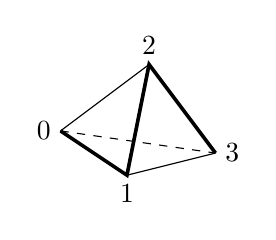
\begin{tikzpicture}[x=40pt,y=40pt]
\draw[line width=1.3pt] (-.7,.1)--(-.1,-.3)--(.1,.7)--(.7,-.1);
\draw (-.7,.1)--(.1,.7);
\draw (-.1,-.3)--(.7,-.1);
\draw[dashed] (-.7,.1)--(.7,-.1);
\draw (-.7,.1) node[anchor=east]{0};
\draw (.7,-.1) node[anchor=west]{3};
\draw (-.1,-.3) node[anchor=north]{1};
\draw (.1,.7) node[anchor=south]{2};
\end{tikzpicture}

Illustration of the subspace $G(3)$ (bold line) embedded in $F(3)$.
\end{center}
The inclusion $\phi^k:G(k)\hookrightarrow F(k)$ induces a map $\phi_k=\Map_{\ssp}(\phi^k,X):\Map_{\ssp}(F(k),X)\to\Map_{\ssp}(G(k),X)$. We can check that
\begin{equation}\label{eq seg con}
\Map_{\ssp}(G(k),X)\cong\holim(X_1\xrightarrow{d_0}X_0\xleftarrow{d_1}X_1\xrightarrow{d_0}\cdots\xrightarrow{d_0}X_0\xleftarrow{d_1}X_1)
\end{equation}
with $k$ copies of $X_1$.

\begin{defin}
We say that a simplicial space $X$ satisfies the Segal condition if $\phi_k:\Map_{\ssp}(F(k),X)\to\Map_{\ssp}(G(k),X)$ is a weak equivalence for each $k\ge 2$.
\end{defin}

Therefore, simplicial spaces satisfying the Segal condition are defined up to weak equivalence by their 0-th and 1-st spaces.

We can define a simplicial enriched structure associated to a simplicial space satisfying the Segal condition:
\begin{defin}\label{simpcat}
Let $W$ be a simplicial space. Define $\Ob W=(W_0)_0$ to be the vertices of $W_0$ and for any $x,y\in\Ob W$, we define $\map_W(x,y)$ to be the fiber of the map $(d_1,d_0):W_1\to W_0\times W_0$ at the point $(x,y)\in W_0\times W_0$. The identity map is defined to be $\id_x=s_0x\in\Map_W(x,x)$.
\end{defin}
However, for a general simplicial space $W$, it is difficult to verify the Segal condition since (\ref{eq seg con}) is given by a homotopy limit. Furthermore, $\map_W(x,y)$ is not fibrant, so we cannot define a homotopy equivalence on the simplicial set. However, requiring $\map_W(x,y)$ to be fibrant for all $(x,y)$ (eg. by requiring $(d_1,d_0):W_1\to W_0\times W_0$ to be a fibration) is still not sufficient. We also want the following condition: we want a homotopy relation that is well-defined up to changing of the end points by a path in $(W_0)_1$, that is, if $[x],[y]\in\pi_0(W_0)$ are the path-components of $x$ and $y$, then we want $\map_W([x],[y])$ to be defined in some way and a homotopy equivalence relation on it.

It turns out that imposing Reedy fibrancy is sufficient.
\begin{defin}
A Segal space is a Reedy fibrant simplicial space satisfying the Segal condition.
\end{defin}
If $W$ is Reedy fibrant, then (\ref{eq seg con}) can be computed as a limit (not just a homotopy limit). Furthermore, since $\ssp$ is proper, the map $\phi_k$ is a fibration for all $k$. Similarly, $d_0,d_1:W_1\to W_0$ are fibrations, hence $(d_1,d_0):W_1\to W_0\times W_0$ is a fibration and $\map_W(x,y)$ are fibrant. Furthermore, $W_1\times_{W_0}\cdots\times_{W_0}W_1$ is a homotopy fibre product. In particular, $W_0$ is fibrant as $W$ is fibrant, and compositions of the fibrant maps in the previous paragraph gives us that $W_k$ is fibrant for all $k$.

\begin{eg}
Every discrete simplicial space ($W_k$ is discrete for each $k$) is Reedy fibrant. Hence, it is a Segal space iff it satisfies the Segal condition. Indeed, if a discrete simplicial space satisfies the Segal condition, then $\phi_k$ will be isomorphisms.
\end{eg}

\subsection{Examples of Segal spaces}\label{egss}
\subsubsection{Classifying space of categories}
We denote by $\mathrm{nerve}(C)$ the nerve of a category $C$, that is, the simplicial set with $n$-simplices given by a chain of composable morphisms
$$c_0\to\ldots\to c_n.$$
\begin{prop}\label{nerve}
$\mathrm{nerve}([n])=\Delta^n$. For any categories $C$ and $D$, there are natural isomorphism $\mathrm{nerve}(C\times D)\cong\mathrm{nerve}(C)\times\mathrm{nerve}(D)$ and $\mathrm{nerve}(D^C)\cong\mathrm{nerve}(D)^{\mathrm{nerve}(C)}$. The nerve functor gives a full embedding $\mathrm{nerve}:\Cat\to\sset$.
\end{prop}

Let $C$ be a category and $W\subset C$ a subcategory such that $\Ob W=\Ob C$.

\begin{defin}
Let $(C,W)$ be a category with its subcategory of weak equivalences. We say that a morphism $f$ is a \textbf{weak equivalence} if $f\in W$.

Let $D$ be any other category. For any two functors $f,g\in C^D$, we say that a natural transformation $f\xrightarrow{\alpha}g$, we say that $\alpha$ is a \textbf{weak equivalence} if $\alpha d \colon f(d) \to g(d)$ is a weak equivalence for all $d\in\Ob D$. Let $\mathrm{we}(C^D)\subset C^D$ be the subcategory of all weak equivalences.

The \textbf{classifying space} of $(C,W)$ is defined to be the simplicial space $N(C,W)$ where
\[
N(C,W)_m=\mathrm{nerve}\,\mathrm{we}(C^{[m]}).
\]
\end{defin}
It is convenient to view an $n$-simplex of $N(C,W)_m$ as a diagram
\begin{equation}\label{visualncw}
\begin{matrix} c_{00}&\to&\cdots&\to&c_{0m}\\\downarrow&&&&\downarrow\\\vdots&&&&\vdots\\\downarrow&&&&\downarrow\\c_{n0}&\to&\cdots&\to&c_{nm}
\end{matrix}
\end{equation}
where the vertical arrows are weak equivalences.

We consider some special cases:
\begin{eg}\label{nerveeg}
\begin{enumerate}
\item Let $C_0\subset C$ be the subcategory consisting of all objects and only the identity morphisms. Then, $\mathrm{discnerve}\,C=N(C,C_0)$ is known as the \textbf{discrete nerve}. In particular $\mathrm{discnerve}([n])=F(n)$. However, note that equivalent categories may not give weakly-equivalent discrete nerves. For example, a single point category with only the identity morphism and a two point category with a unique isomorphism between the two points have non-equivalent discrete nerves.

\item Let $\mathrm{iso}\,C\subset C$ be the subcategory consisting of all objects and all invertible morphisms in $C$ (i.e. the maximal subgroupoid of $C$). The \textbf{classifying space} of $C$ is defined to be $NC=N(C,\mathrm{iso}\,C)$.
\end{enumerate}
\end{eg}

\begin{prop}
The classifying spaces $\mathrm{discnerve}\,C$ and $NC$ of a category $C$ are Segal spaces.
\end{prop}
\begin{proof}
Using the representation of an $n$-simplex in $N(C,W)_m$ by the diagram in (\ref{visualncw}), we easily see that there is a natural isomorphism $N(C,W)_m\cong N(C,W)_1\times_{N(C,W)_0}\cdots\times_{N(C,W)_0}N(C,W)_1$.

Since all discrete simplicial spaces are Reedy fibrant, thus $\mathrm{discnerve}\,C$ is a Segal space.

To show that $NC$ is Reedy fibrant, we need to show that the maps $l_m:NC_m\to\partial NC_m$ are fibrations for $m\ge0$. They are easy to check using the representation of $n$-simplices in $NC_m$ by (\ref{visualncw}). Indeed, $l_m$ is an isomorphism for $m\ge 3$.
\end{proof}

We obtain a result similar to Prop.~\ref{nerve}:
\begin{prop}\label{nerveprop}
Let $C$ and $D$ be categories. There are natural isomorphisms $N(C\times D)\cong NC\times ND$ and $N(D^C)\cong ND^{NC}$. More generally, given $\mathrm{iso}\,D\subset W\subset D$ a subcategory,
\begin{equation} \label{nfuncat}
N(D^C,\mathrm{we}(D^C))\cong N(D,W)^{NC}\cong N(D,W)^{\mathrm{discnerve}\,C}.
\end{equation}
The functor $N:\Cat\to \ssp$ is a full embedding of categories. $F:C\to D$ is an equivalence of categories iff $NF$ is a weak equivalence of simplicial spaces.
\end{prop}
\begin{proof}
See \cite[Thm 3.7, Prop 3.11]{rezk}.
\end{proof}

\subsubsection{Classifying space of a closed model category}
Let $C=M$ be a closed model category and $W\subset M$ be its subcategory of weak equivalences. As noted above, we have a simplicial space $N(C,W)$. $N(C,W)$ is in general not Reedy fibrant. However, we can take a functorial Reedy fibrant replacement of it, for example, by the small object argument. Note that taking a Reedy fibrant replacement does not change the homotopy type of the spaces in each degree.

\begin{defin}
The classifying space of a simplicial close model category $(M,W)$ is a functorial Reedy fibrant replacement $N^f(M)$ of $N(M,W)$.
\end{defin}

As most of the model categories we are interested in are not small, we need to be take care of some set theoretical considerations. However, we can always work in a larger universe, so $N^f(M)$ may not be in the same universe as $M$.

\begin{thm}
$N^f(M)$ is a Segal space.
\end{thm}
\begin{proof}
See \cite[Thm 8.3]{rezk}.
\end{proof}

Note that any category $C$ with finite limits and colimits can be given a model structure in which the weak equivalences are exactly the isomorphisms. In this case, $N(C,W)=N(C,\mathrm{iso}\,C)$ is already a Segal space, so $N^f(C)=NC$. However, in general, it is difficult to compute the Reedy fibrant replacement of a simplicial space, and thus the classifying space. Later, we will show another way to obtain the classifying space through a localisation functor.

Given a small indexing category $I$, we can define a subcategory of weak equivalence $\mathrm{we}(M^I)\subset M^I$. (\ref{nfuncat}) and the Reedy fibrant replacement functor induces a natural map
$$f:N(M^I,\mathrm{we}(M^I))\cong N(M,W)^{\mathrm{discnerve}\,I}\to N^f(M)^{\mathrm{discnerve}\,I}.$$
In general, the map $f$ is not a weak equivalence, but a result by Dwyer and Kan says that, in some special cases, for example if $M$ is cofibrantly generated, $f$ is a weak equivalence. In that case, we see that the homotopy type of the classifying space of the functor category $M^I$ is entirely determined by the homotopy type of $M$. More precisely, we state the following theorem by Dwyer and Kan.
\begin{thm}[Strictification theorem]
Suppose $J$ is a small indexing category and $M=\sset^J$, then the map $f:N(M^I,\mathrm{we}(M^I))\to N^f(M)^{\mathrm{discnerve}\,I}\cong N^f(M)^{NI}$ is a weak equivalence. In particlar, it induces a weak equivalence of Segal spaces $N^f(M^I)\to N^f(M)^{NI}$.
\end{thm}
\begin{proof}
See \cite[Thm 8.11]{rezk}.
\end{proof}

\subsection{Homotopy theory in Segal spaces and categories}
Recall the construction of a simplicial enriched structure associated to a Segal space, given in Def. \ref{simpcat} (It may not a simplicial enriched category since associativity may not be strict). That construction allows us to construct the homotopy category associated to the Segal space.

We begin by defining homotopic morphisms.
\begin{defin}
Let $W$ be a Segal space and $x,y\in\Ob W$. Two maps $f,g\in\map(x,y)$ are homotopic if they lie in the same path component of $\map(x,y)$, i.e., $[f]=[g]\in\pi_0\map(x,y)$.
\end{defin}

In general, given $k+1$ objects $x_0,\to,x_k\in\Ob W$, we can define $\map_W(x_0,\to,x_k)$ to be the fibre of the fibration $(\alpha_0,\ldots,\alpha_n):W_k\to W_0^k$ at the point $(x_0,\ldots,x_k)$, where $\alpha_i$ is the map induced by $\alpha^i:[0]\to[k]$ taking 0 to $i$. The fibre of the commutative diagram

\centerline{\xymatrix{W_k\ar[rr]^{\sim}_{\phi_k}\ar[dr]_{(\alpha_0,\ldots,\alpha_n)}&&W_1\times_{W_0}\cdots\times_{W_0}W_1\ar[dl]\\
&W_0^{k+1}}}

induces a trivial fibration
$$\phi_k:\map(x_0,\ldots,x_k)\to\map(x_0,x_1)\times\cdots\times\map(x_{n-1},x_n).$$

We can thus define composition of maps up to homotopy.
\begin{defin}
If $f\in\map(x,y)$ and $g\in\map(y,z)$, we define $g\circ f=d_1h$ for some $h\in\map(x,y,z)$ such that $\phi_2(h)\sim(f,g)$ are homotopic.
\end{defin}

\begin{prop}
For each Segal space $W$, we have an associated homotopy category $\Ho W$ where $\Ob\Ho W=\Ob W$ and $\map_{\Ho W}(x,y)=\pi_0\map_W(x,y)$.
\end{prop}
\begin{proof}
It suffices to show that $f\circ(g\circ h)\sim(f\circ g)\circ h$ and $f\circ\id\sim f\sim\id\circ f$. See \cite[Prop 5.4]{rezk} for details.
\end{proof}

\begin{eg}
Let $C$ be a category. Then, $\Ob NC=\Ob C$ and $\map_{NC}(x,y)\cong\hom_C(x,y)$ is the discrete simplicial set generated by elements of $\hom_C(x,y)$. Thus, $\Ho NC\cong C$.
\end{eg}

Now, we define the notion of homotopy equivalence. Let $Z(3)=\mathrm{discnerve}(0\to2\leftarrow1\to3)\subset F(3)$. It induces a fibration $W_3\to\Map_{\ssp}(Z(3),W)\cong W_1\times_{W_0}W_1\times_{W_0}W_1$.

\begin{prop}
Let $g\in\map_W(x,y)$. The following statements are equivalent:
\begin{enumerate}
\item There exist $f,h\in\map_W(y,x)$ such that $g\circ f\sim\id_y$ and $h\circ g\sim\id_x$.
\item $(\id_x,g,\id_y)\in\Map_{\ssp}(Z(3),W)$ admits a lift to some $H\in W_3$.
\end{enumerate}
\end{prop}
\begin{proof}
Easy check.
\end{proof}

If $g$ satisfies either of the above equivalent statements, we call $g$ a \textbf{homotopy equivalence}.

\begin{lemma}
If $g\in (W_1)_0$ is a vertex connected by a path in $(W_1)_1$ to a vertex $g'$, then $g$ is a homotopy equivalence iff $g'$ is one.
\end{lemma}
\begin{proof}
See \cite[Lemma 5.8]{rezk}.
\end{proof}

\begin{defin}
We can thus define the space of homotopy equivalence to be the components $W_{\mathrm{hoequiv}}\subset W_1$ of homotopy equivalences.
\end{defin}
Note that $s_0:W_0\to W_1$ factors through $W_{\mathrm{hoequiv}}$ since $s_0x=\id_x\in W_{\mathrm{hoequiv}}$ for all $x\in W_0$.

\subsection{Complete Segal spaces}
We have now defined Segal spaces and their homotopy categories. However, there are too many Segal spaces with respect to other models of $(\infty,1)$-categories. See Example \ref{nervecomplete} below.
We define the following:
\begin{defin}
A complete Segal space is a Segal space such that the map $s_0:W_0\to W_{\mathrm{hoequiv}}$ is a weak equivalence.
\end{defin}

We want to find an object in $\ssp$ that represents the functor $W\mapsto W_{\mathrm{hoequiv}}$, at least up to weak equivalence. Let $E=\mathrm{discnerve}(I[1])$. We have the following theorem:
\begin{thm}\label{rephoequiv}
The map $\Map_{\ssp}(E,W)\to W_1$ induced by the inclusion $F(1)\hookrightarrow E$ factors through $W_{\mathrm{hoequiv}}\subset W_1$, and induces a weak equivalence $\Map_{\ssp}(E,W)\to W_{\mathrm{hoequiv}}$.
\end{thm}
\begin{proof}
The proof is technical. See \cite[Thm 6.2]{rezk}.
\end{proof}

Some corollaries of the theorem include
\begin{cor}\label{rephoequivcor}
Let $W$ be a Segal space. The following are equivalent:
\begin{enumerate}
\item $W$ is a complete Segal space.
\item The map $W_0\to\Map_{\ssp}(E,W)$ induced by $E\to F(0)$ is a weak equivalence.
\item For each pair $x,y\in\Ob W$, the fibre $\mathrm{hoequiv}(x,y)$ of the fibration $W_{\mathrm{hoequiv}}\xrightarrow{(d_1,d_0)} W_0\times W_0$ is naturally weak equivalent to the space of paths in $W_0$ from $x$ to $y$.
\end{enumerate}
\end{cor}
\begin{proof}
$(i)\Leftrightarrow(ii)$ is clear from Thm.~\ref{rephoequiv}.

$(ii)\Leftrightarrow(iii)$: consider the composition $\Delta:W_0\xrightarrow{s_0}W_{\mathrm{hoequiv}}\xrightarrow{(d_1,d_0)} W_0\times W_0$. Since $(d_1,d_0)$ is a fibration, $\mathrm{hoequiv}(x,y)$ is actually a homotopy fibre (Prop.~\ref{hompullback}). The spcae of paths in $W_0$ from $x$ to $y$ is the homotopy fibre of $\Delta$.
\end{proof}

\begin{cor}
Let $\Ob W/\sim$ denote the set of homotopy equivalence classes of objects in $\Ho W$. If $W$ is a complete Segal space, then $\pi_0W_0\cong\Ob W/\sim$.
\end{cor}
\begin{proof}
Follows immediately from (iii) of the previous corollary.
\end{proof}

\begin{eg}
The classifying space $N(C)$ for a category $C$ and the classifying space $N^f(M)$ for a simplicial closed model category $M$ are complete Segal spaces. See \cite{rezk} for details of the proofs. $\mathrm{discnerve}\,(C)$ is not complete.
\end{eg}

\begin{defin}
Let $W$ be a Segal space, we define the completion of $W$ to be a complete Segal space $\hat W$ with a map $i_W:W\to\hat W$ which is universal among all maps from $W$ to a complete Segal space.
\end{defin}

\begin{prop}
There exists a completion functor given by $i_W:W\to\hat W$ on the category of Segal spaces.
\end{prop}
\begin{proof}
Let $E(m)=\mathrm{discnerve}(I[m])$. For each $n \ge 0$, we can define a simplicial set $\tilde W_n=\diag([m]\mapsto (W^{E(m)})_n \cong \Map_{\ssp}(E(m)\times F(n),W))$ where the diagonal map $\diag \colon \ssp\cong\sset^{(2)}\to\sset$ is that induced by $[n]\mapsto[n]\times[n]$. The face and degeneracy maps induced from $d^i \colon F(n)\to F(n+1)$ and $s^i \colon F(n)\to F(n-1)$ gives us a simplicial space $\tilde W$ with a natural map $W\to \tilde W$. $\hat W$ is defined to be a functorial Reedy fibrant replacement of $\tilde W$, thus inducing a map $i_W:W\to\tilde W\to\hat W$.

For the details of the proof, see \cite{rezk}.
\end{proof}

In general, the above construction of the completion of a Segal space is not easy to understand.

\begin{eg}\label{nervecomplete}
Given a category $C$, $\mathrm{discnerve}\,C$ is a Segal space, but not complete. Its completion $\widehat{\mathrm{discnerve}\,C}=NC$. As mentioned in Example \ref{nerveeg}, equivalent categories may give rise to non-weakly equivalent discrete nerves, but we see that the completions are weakly equivalent iff the categories are equivalent (Prop.~\ref{nerveprop}).
\end{eg}

\subsection{Closed model category structures related to Segal spaces}
In this section, we will introduce two other model category structures on the category of simplicial spaces $\ssp$. The fibrant-cofibrant objects will be the Segal spaces and the complete Segal spaces in the two structures respectively. We will also show the relationship between weak equivalences in these two structures and with Reedy weak equivalences.

\begin{thm}
There exists a closed model category structure on $\ssp$ with the following properties:
\begin{enumerate}
\item The cofibrations are the monomorphisms.
\item The weak equivalences are maps $f$ such that $\Map_{\ssp}(f,W)$ is a weak equivalence for all Segal spaces $W$.
\item The fibrations are the maps that satisfy the right lifting property with respect to all trivial cofibrations.
\end{enumerate}
This is called the \textbf{Segal space model category structure} on $\ssp$, an is denoted as $\mathcal{SS}$. This model structure is compatible with the cartesian closed standard model structure on $\sset$. All objects are cofibrant and the fibrant objects are precisely the Segal spaces. A Reedy weak equivalence between two objects $X,Y$ is a weak equivalence in $\mathcal{SS}$ and the converse is true if $X,Y$ are Segal spaces.
\end{thm}
\begin{proof}
$\mathcal{SS}$ is the left Bousfield localisation of the Reedy model category structure with respect to the set of maps $S=\{G(k)\hookrightarrow F(k)\}$. See \cite[Thm 7.1]{rezk} for the proof of the compatibility with cartesian closure.
\end{proof}

\begin{thm}
There exists a closed model category structure on $\ssp$ with the following properties:
\begin{enumerate}
\item The cofibrations are the monomorphisms.
\item The weak equivalences are maps $f$ such that $\Map_{\ssp}(f,W)$ is a weak equivalence for all complete Segal spaces $W$.
\item The fibrations are the maps that satisfy the right lifting property with respect to all trivial cofibrations.
\end{enumerate}
This is called the \textbf{complete Segal space model category structure} on $\ssp$, an is denoted as $\mathcal{CSS}$. This model structure is compatible with the cartesian closed standard model structure on $\sset$. All objects are cofibrant and the fibrant objects are precisely the complete Segal spaces. A Reedy weak equivalence between two objects $X,Y$ is a weak equivalence in $\mathcal{CSS}$ and the converse is true if $X,Y$ are complete Segal spaces.
\end{thm}
\begin{proof}
By Cor.~\ref{rephoequivcor}, we see that $\mathcal{CSS}$ is the left Bousfield localisation of $\mathcal{SS}$ with respect to the map $E\to F(0)$. See \cite[Thm 7.2]{rezk}for the proof of the compatibility with cartesian closure.
\end{proof}

Let $\Ho\mathcal{SS}$ and $\Ho\mathcal{CSS}$ be the homotopy categories associated to the two model structures respectively, and $\Ho\mathcal{SS}_{cf}$ and $\Ho\mathcal{CSS}_{cf}$ denote the respective full subcategories of fibrant-cofibrant objects, namely the Segal spaces and the complete Segal spaces respectively.

Note that for any model category $M$, the inclusion $M_{cf}\subset M$ induces an equivalence of homotopy categories $\Ho M_{cf}\cong\Ho M$. This, in particular, implies that small homotopy limits and colimits exist in the subcategory $M_{cf}$.

An immediate consequence of the compatibility of these model structures with cartesian closure is that if $W$ is a (complete) Segal space and $X$ is a simplicial space, then $W^X$ is a (complete) Segal space. In particular, given any two complete Segal spaces $X$ and $Y$, we have a natural $(\infty,1)$-category structure on the functors from $X$ to $Y$ given by the internal-hom object $Y^X$.

To understand the relationship between the two model category structures, we introduce the notion of Dwyer-Kan equivalence.
\begin{defin}
A map $f:U\to V$ between two Segal spaces is a Dwyer-Kan equivalence if
\begin{enumerate}
\item the induced map $\Ho f:\Ho U\to\Ho V$ is an equivalence of categories; and
\item for each pair of objects $x,x'\in U$, the induced function $\map_U(x,x')\to\map_V(fx,fx')$ is a weak equivalence.
\end{enumerate}
An equivalent formulation of condition (i) is
\begin{enumerate}
\item the induced map $\Ob U/\sim\to\Ob V/\sim$ is a bijection on the equivalence classes of objects.
\end{enumerate}
\end{defin}
We have the following theorem
\begin{thm}\label{thm dk reedy}
Let $f:U\to V$ be a map of Segal spaces. Then $f$ is a Dwyer-Kan equivalence iff $f$ is a weak equivalence in $\mathcal{CSS}$. If, in addition, $U$ and $V$ are complete Segal spaces, then $f$ is a Dwyer-Kan equivalence iff $f$ is a Reedy weak equivalence.
\end{thm}
\begin{proof}
See \cite[Thm 7.7]{rezk}.
\end{proof}

We thus have the following series of implications for simplicial spaces
$$\xymatrix{\text{Reedy w.e.}\ar@{==>}@/_.3pc/[r]_{\text{Segal sp.}}&\text{w.e. in }\mathcal{SS}\ar@{==>}@/_.3pc/[r]_{\text{c. Segal sp.}}\ar@{=>}@/_.3pc/[l]&\text{w.e. in }\mathcal{CSS}\ar@{<=>}[r]_{\text{Segal sp.}}\ar@{=>}@/_.3pc/[l]&\text{DK-equiv.}}$$

The proof of Thm.~\ref{thm dk reedy} relies on the following proposition, which we will state as it is also of interest on its own.
\begin{prop}\label{iw}
The completion functor $i_W:W\to\widehat W$ is a Dwyer-Kan equivalence and a weak-equivalence in $\mathcal{CSS}$.
\end{prop}
\begin{proof}
See \cite[Sec.~14]{rezk}.
\end{proof}

\begin{cor}
If $f:U\to V$ map of Segal spaces is a weak equivalence in $\mathcal{SS}$, then $\hat f:\hat U\to\hat V$ is a weak equivalence in $\mathcal{CSS}$. Thus, the completion functor induces a well-defined functor between the homotopy categories $i:\Ho\mathcal{SS}_{cf}\to\Ho\mathcal{CSS}_{cf}$.
\end{cor}
\begin{proof}
This follows immediately from Prop.~\ref{iw} and the fact that a weak equivalence in $\mathcal{SS}$ is a weak equivalence in $\mathcal{CSS}$.
\end{proof}

\subsection{Classifying spaces: another perspective}\label{sslocal}
To end of this section, we return to the example of the classifying space of a category $C$ with weak equivalences $W$. The ideas for this section are derived from the notes of a talk by To\"en \cite{toentalksegal}. The following diagram of categories
\begin{equation} \label{seglocalpushout}
\xymatrix{\coprod_{f\in W}[1]\ar[r]^{\sqcup i}\ar[d]&\coprod_{f\in W}I[1]\\C}
\end{equation}
induces a pushout square in $\ssp$ of the classifying spaces
\[
\xymatrix{
\coprod_{f \in W} F(1)\ar[r]^{\sqcup N(i)}\ar[d] & \coprod_{f\in W} N(I[1]) \ar[d] \\ NC\ar[r]&\tilde N(C,W)
}.
\]
Since $\sqcup i$ is a cofibration and all objects are cofibrant in $\mathcal{CSS}$, the square is also a homotopy pushout (see \cite[Prop A.2.2.4]{htt}). Since $\mathcal{CSS}_{cf}$ is closed under homotopy pushouts, there exists $\hat N(C,W)\in\mathcal{CSS}_{cf}$ such that $\hat N(C,W)$ is weakly equivalent to $\tilde N(C,W)$ and
$$\xymatrix{\coprod_{f\in W}F(1)\ar[r]^{\sqcup N(i)}\ar[d]&\coprod_{f\in W}N(I[1])\ar[d]\\NC\ar[r]&\hat N(C,W)}$$
is a homotopy pushout square in $\mathcal{CSS}_{cf}$.

If $W\subset\mathrm{iso}\,C$, there exists a lift
$$\xymatrix{\coprod_{f\in W}F(1)\ar[r]^{\sqcup N(i)}\ar[d]&\coprod_{f\in W}N(I[1])\ar[d]\ar@{-->}[dl]_{\exists}\\NC\ar[r]&\hat N(C,W)},$$
so $\hat N(C,W)=NC$.

We have the following result:
\begin{prop}
Suppose $W\supset\mathrm{iso}\,C$, then $\hat N(C,W)=\widehat{N(C,W)^f}$ is the Segal completion of a functorial fibrant replacement of $N(C,W)$.
\end{prop}
\begin{proof}
Let $N([1],[1])$ be a classifying space of $C=[1]$ with all morphisms regarded as weak equivalences. Then, it is clear that the following is a homotopy pushout square:
$$\xymatrix{\coprod_{f\in W}F(1)\ar[r]^{\sqcup N(i)}\ar[d]&\coprod_{f\in W}N([1],[1])\ar[d]\\NC\ar[r]&N(C,W)}.$$
The natural inclusion $N([1],[1])\subset N(I[1])$ is a Reedy weak equivalence. This is because, for every $m\ge 0$, $\mathrm{nerve}\,\mathrm{we}([1]^{[m]})\to\mathrm{nerve}\,\mathrm{iso}(I[1]^{[m]})$ induces a weak equivalence since their geometric realisations are both contractible.

Hence, the homotopy pushout induces a weak equivalence $N(C,W)\xrightarrow\sim\hat N(C,W)$.
\end{proof}

Hence, in the case where $C=M$ is a model category and $W$ is the set of weak equivalences, we get $\hat N(M,W)=N^f(M)$, the classifying space we previously defined.


\section{Segal Categories}
While complete Segal spaces are good models of weak $(\infty,1)$-categories, a key disadvantage is that they are difficult to construct. In most constructions, we obtain a Segal space that is not complete. The completion functor is abstract and difficult to compute in practice. To overcome this problem, another model, the Segal categories, was developed. Segal categories avoid the cumbersome procedure of completion by imposing an additional condition on the simplicial spaces we are considering (that the 0-space is discrete).

Segal categories were formally defined by Dwyer, Kan and Smith in \cite{dks}. They were used extensively and generalised to $n$-Segal categories by Hirschowitz and Simpson in their studies of $n$-stacks \cite{hs}. In this section, we will follow the ideas in \cite{hs} but refer to the work of Bergner \cite{bergner2} for more explicit constructions.

\subsection{Segal precategories, categories and closed model structure}
\begin{defin}
A simplicial space $X$ is a Segal precategory if $X_0$ is discrete. Let $\mathcal{PC}at$ be the category of Segal pre-categories. A Segal precategory $X$ that satisfies the Segal condition (\ref{segal}) is called a Segal category.
\end{defin}

\begin{eg}
Let $C$ be any category, then $\mathrm{discnerve}\,C$ is a Segal category. Note that under the model category structure that we are going to impose on $\mathcal{PC}at$, $f:C\to D$ is an equivalence of categories iff $\mathrm{discnerve}\,f$ is a weak equivalence (unlike in the Reedy model structure or $\mathcal{SS}$).
\end{eg}

Every simplicial enriched category $C$ can be seen as a Segal precategory, which we will also denote by $C$, by setting $C_0=\Ob C$ and $C_n=\sqcup_{x,y\in\Ob C}(\map_C(x,y))_{n-1}$ with appropriate face and degeneracy maps. Note that, however, a Segal category may not be a simplicial category since associativity is not strict. To obtain a simplicial category, we will need to consider the category generated by the Segal category, which we will not define here.

Recall that given a simplicial space $X$, we can define $\Ob X$ and mapping spaces $\map_X(x,y)$ (Def.~\ref{simpcat}). We denote $x\sim y$ if $\map_X(x,y)\ne\emptyset$. However, $\sim$ may not be an equivalence relation. We denote by the same symbol the equivalence relation generated by $\sim$.

The closed model structure on Segal precategories corresponding to Segal categories cannot be given by any Bousfield localisation. Instead, we need some effort to define a proper notion of weak equivalences. We first construct a functor $L_C:\mathcal{PC}at\to\mathcal{PC}at$ that sends a precategory $X$ into a Segal category $L_CX$. Hirschowitz and Simpsons proved the existence of such a functor (indeed for Segal $n$-categories) in \cite{hs} but we shall give the explicit construction given by Bergner \cite{bergner2}.

We want to construct $L_CX$ as a functorial fibrant replacement of $X$ in the Segal space model category structure $\mathcal{SS}$, in such a way that $L_CX$ is still a precategory. We proceed by the small object argument. We have a set of generating trivial cofibrations in $\mathcal{SS}$ (obtained from the generating trivial cofibrations of the Reedy model structure by localisation):
$$F(k)\times\Lambda^l_t\sqcup_{G(k)\times\Lambda^l_t}G(k)\times\Delta^l\to F(k)\times\Delta^l,\qquad k\ge0,l\ge1,0\le t\le l$$
where $G(0)=\emptyset$. The fibrant replacement can be constructed as a colimit of the iterated pushout
$$\xymatrix{\coprod(F(k)\times\Lambda^l_t\sqcup_{G(k)\times\Lambda^l_t}G(k)\times\Delta^l)\ar[r]\ar[d]&X_i\ar[d]\\
\coprod(F(k)\times\Delta^l)\ar[r]&X_{i+1}}$$
where $X=X_0$ and the coproduct is taken over all maps $F(k)\times\Lambda^l_t\sqcup_{G(k)\times\Lambda^l_t}G(k)\times\Delta^l\to X_i$ with $k\ge 0$, $l\ge 1$ and $0\le t\le l$.

Note that the map on the zero space induced by a generating trivial cofibration is given by $[k]\times\Lambda^l_t\cup[k]\times\Delta^l\cong [k]\times\Delta^l\xrightarrow{\id}[k]\times\Delta^l$ for $k> 0$ and $\Lambda^l_t\to\Delta^l$ for a $k=0$.

The Segal space thus obtained may not have a discrete 0-space, and is thus not a Segal category. To fix this, we exclude the maps with $k=0$ and consider the iterated pushout with respect to the coproduct over the subset of maps with $k>0$. Let $L_CX$ be the colimit of this sequence of pushouts.

\begin{prop}
$L_CX$ as defined above is a functorial fibrant replacement of $X$, so $L_C:\mathcal{PC}at\to\mathcal{PC}at$ is a well-defined functor taking a precategory to a Segal category that is also a Segal space.
\end{prop}

\begin{proof}
By the small object argument, to check that this is indeed a fibrant replacement of $X$ in $\mathcal{SS}$, it suffices to check that $L_CX$ satisfies the RLP with respect to all generating trivial cofibrations with $k=0$. This is equivalent to checking that the lift exists in the following diagram
$$\xymatrix{\Lambda^l_t\ar[r]\ar[d]&\Map_{\ssp}(F(0),L_CX)\cong (L_CX)_0\\\Delta^l\ar@{-->}[ur]}.$$
This is true since $L_CX$ is a discrete simplicial set and hence a Kan complex.
\end{proof}

We remark that in the case where $f:X\to Y$ is a map between two Segal categories which are also Segal spaces, then the two definitions of Dwyer-Kan equivalence are equivalent.

We are now ready to define a closed model category structure on precategories.

\begin{thm}\label{thm pcat model}
There exists a closed model category structure on $\mathcal{PC}at$ in which
\begin{enumerate}
\item the cofibrations are precisely the monomorphisms;
\item the weak equivalences are precisely the maps $f:X\to Y$ such that $L_Cf:L_CX\to L_CY$ is a Dwyer-Kan equivalence of Segal spaces; and
\item the fibrations are maps that satisfy the right lifting property with respect to all trivial cofibrations.
\end{enumerate}
We denote $\mathcal{PC}at$ equipped with this model category structure $\mathcal{SC}$. The fibrant-cofibrant objects of this model structure are precisely the Reedy-fibrant Segal categories.
\end{thm}
\begin{proof}
See \cite[Thm 2.3]{hs} and \cite[Thm 5.1]{bergner2} for two different proofs of the existence of this model structure. See \cite[Cor 5.13]{bergner2} and \cite[Thm 3.2]{bergner3} for the proof of the last statement.
\end{proof}

\begin{rmk}
Thm.~\ref{thm pcat model} and the comparisons between the different models of $(\infty,1)$-categories (Sec.~\ref{sec comp thms}) show that Reedy-fibrant Segal categories give a good model of $(\infty,1)$-categories. Reedy-fibrant Segal categories are easy to construct, avoiding the cumbersome Segal completion procedure required in defining complete Segal spaces. However, to verify that two Segal categories are equivalent, we still need to pass through the complete Segal spaces.
\end{rmk}

Let $\mathrm{SeCat}\subset\mathcal{SC}$ and $\Ho\mathrm{SeCat}\subset\Ho\mathcal{SC}$ be the full subcategories of Segal categories. Since $\mathrm{SeCat}$ contains all fibrant-cofibrant objects, $\Ho\mathrm{SeCat}\cong\Ho\mathcal{SC}$ and in particular contains all small homotopy limits and colimits.

\subsection{Segal localisation}
We want to construct a localisation similar to that in Section \ref{sslocal}. Let $C$ be a category and $W\subset C$ be a subcategory of weak equivalences. Taking discrete nerves on the diagram of categories (\ref{seglocalpushout}), we obtain a pushout diagram in $\mathcal{SC}$:
$$\xymatrix{\coprod_{f\in W}F(1)\ar[r]\ar[d]&\coprod_{f\in W}E\ar[d]\\\mathrm{discnerve}\,C\ar[r]&\tilde C}.$$
Since the top arrow is a cofibration and all objects are cofibrant, it is a homotopy pushout square as well. Hence, there exists $L(C,W)\in\mathrm{SeCat}$ (indeed, we can even choose $L(C,W)\in\mathcal{SC}_{cf}$ the subcategory of Reedy-fibrant Segal categories) such that $L(C,W)$ is weakly equivalent to $\tilde C$ and the following diagram is a homotopy pushout square in $\mathrm{SeCat}$:
$$\xymatrix{\coprod_{f\in W}F(1)\ar[r]\ar[d]&\coprod_{f\in W}E\ar[d]\\\mathrm{discnerve}\,C\ar[r]&L(C,W)}.$$

Note that since the completion functor commutes with colimits and $\widehat{\mathrm{discnerve}\,C}\cong NC$, we have that $\widehat{L(C,W)}\cong\hat N(C,W)$.

If $W=\mathrm{iso}\,C$, we get $LC=\mathrm{discnerve}\,C$ as seen in Section \ref{sslocal}.

In \cite{dkcomputing}, Dwyer and Kan showed that $L(C,W)$ can be explicitly constructed using the hammock localisation $L^H(C,W)$ (see also Chap.~\ref{chapter:simplicial-localization}).

Let $M$ be a simplicial closed model category, with weak equivalences $W$. Let $M_{cf}\subset M$ be the simplicial subcategory. Dwyer and Kan proved the following result:

\begin{thm}
Let $M$ be a closed simplicial model category. Then, $LM=L(M,W)\cong L^HM\cong M_{cf}$ are weakly equivalent.
\end{thm}
\begin{proof}
See \cite{dkfunction}.
\end{proof}

This theorem allows us to compute the localisation of simplicial model categories easily.
\begin{eg}
\begin{enumerate}
\item Let $M=\sset$ be the category of simplicial sets with the usual model structure, then $M_{cf}$ is the subcategory of Kan complexes. $M_{cf}$ satisfies the Segal condition since homotopy is an equivalence relation on Kan complexes. Hence, $L\sset$ gives us the theory of Kan complexes (or equivalently CW-complexes) as an $(\infty,1)$-category.
\item Let $M=\mathrm{Top}$ be the category of topological spaces, then $L\mathrm{Top}\cong\mathrm{Top}_{cf}$ is the subcategory of CW-complexes. Hence, we see that the localisation of $\sset$ and $\mathrm{Top}$ give the same Segal category.
\item Let $M=\ssp$ with the Reedy model structure. We thus get $L\ssp$ as the Segal category of all Reedy-fibrant simplicial spaces. If we equip the simplicial spaces with the (complete) Segal space model structure, we get $L\mathcal{SS}$ ($L\mathcal{CSS}$) the Segal category of all (complete) Segal spaces.
\item Let $M=\mathcal{SC}$, then $L\mathcal{SC}$ is the Segal category of all Segal categories (up to some change in universe).
\end{enumerate}
\end{eg}
We see that Segal localisation gives us a $(\infty,1)$-category of $(\infty,1)$-categories. As in the case of complete Segal spaces, we have a strictification theorem.

\begin{thm}[Strictification theorem]
Let $M$ be a cofibrantly generated simplicial model category and $I$ a small category, then we have a weak equivalence of Segal categories (Dwyer-Kan equivalence)
$$L(M^I)\cong L(M)^{\mathrm{discnerve}\,I}.$$
\end{thm}
\begin{proof}
See \cite{hs} and \cite{tv}.
\end{proof}

In particular, this implies that to compute small limits and colimits of (complete) Segal spaces or Segal categories, it suffices to compute the homotopy limits and colimits in the larger categories of simplicial spaces or precategories. The strictification theorem also gives a form of Yoneda's lemma for $(\infty,1)$-categories. See To\"en and Vezzosi's paper \cite{tv} for more details.


\section{Comparison theorems}\label{sec comp thms}
In this section, we will show that complete Segal spaces, Reedy-fibrant Segal categories and quasi-categories are equally valid models for $(\infty,1)$-categories. To this end, we will state a number of comparison theorems between complete Segal spaces, Segal categories and other models of $(\infty,1)$-categories.

The main mechanism in proving the equivalence of two model categories is Quillen equivalence (Sec.~\ref{subsec Quillen adjunction}). Recall that a Quillen equivalence of model categories induces an adjoint equivalence of the underlying homotopy categories (Thm.~\ref{thm quillen adjuntion}).
This implies that if we have a Quillen equivalence between two models of infinity categories, they have the same objects up to weak equivalences and their full subcategories of fibrant-cofibrant objects are homotopy equivalent (which is the best we can expect to ask for).

We have the following diagram of Quillen equivalences.
$$\xymatrix{\mathcal{CSS}\ar@/^/[dr]&\mathcal{SC}\ar[l]\ar@/^/[d]&\mathcal{SC}'\ar[l]\ar[r]&s\mathcal{C}\\
&\mathcal{QC}\ar@/^/[ul]\ar@/^/[u]\ar[urr]}$$
An arrow in the diagram refers to the direction of the left adjoint. $\mathcal{QC}$ is the category of simplicial sets with the Joyal model category structure, $s\mathcal{C}$ is the category of simplicial enriched categories and $\mathcal{SC}'$ is another model structure on precategories.

We shall only present the Quillen equivalences among $\mathcal{CSS}$, $\mathcal{SC}$ and $\mathcal{QC}$. We refer to Bergner's paper \cite{bergner3} for the construction of the fibrant model category structure $\mathcal{SC}'$ on precategories (as opposed to the cofibrant structure $\mathcal{SC}$). It was constructed to proved the equivalence with $s\mathcal{C}$. The equivalence between $\mathcal{SC}$ and $\mathcal{SC}'$ is given by the identity functor. For the equivalence between simplicial categories and quasi-categories, we refer to \cite{joyal3}.

In this section, we will not present the proofs, but instead just sketch the construction of the functors or model structures.

\subsection{Some model category structures}
First we construct the three model category structures that we have yet to construct.

\begin{defin}
Let $X$ be a simplicial set, for any $x,y\in X_0$, we write $x\sim y$ if there exists $w\in X_1$ such that $d_1w=x$ and $d_0w=y$. we define $\tau_0X$ be the set of equivalence class in $X_0$ under the equivalence relation generated by $\sim$.

Let $X(x,y)$ be the fibre of the projection $X^I\xrightarrow{(d_1,d_0)} X\times X$.

Let $f:X\to Y$ be a map of simplicial sets, we say that $f$ is essentially surjective if the induced map $\tau_0X\to\tau_0Y$ is surjective. We say that $f$ is fully faithful if for every pair $x,y\in X_0$, the induced map $X(x,y)\to Y(fx,fy)$ is a weak equivalence (under the standard model category structure). We say that $f$ is a weak categorical equivalence if $f$ is both essentially surjective and fully faithful.
\end{defin}
\begin{thm}
There is a closed model category structure on $\sset$, which we will denote as $\mathcal{QC}$, the quasi-category model structure, in which
\begin{enumerate}
\item the cofibrations are precisely the monomorphisms;
\item the weak equivalences are precisely the weak categorical equivalences; and
\item the fibrations are maps satisfying the right lifting property with respect to trivial cofibrations.
\end{enumerate}
The fibrant-cofibrant objects in this model structure are precisely the quasi-categories.
\end{thm}

\begin{proof}
See \cite{joyal2}.
\end{proof}

Next we define a closed model category structure on simplical categories.
\begin{thm}
There is a closed model category structure on $s\mathcal{C}$, in which
\begin{enumerate}
\item the weak equivalences are the Dwyer-Kan equivalences;
\item the fibrations are maps $F:C\to D$ satisfying:
\begin{itemize}
\item for any $x,y\in C$, the induced map $\map_C(x,y)\to\map_D(Fx,Fy)$ is a fibration of simplicial sets;
\item for any $x_1\in C$, $y\in D$ and homotopy equivalence $e:Fx_1\to y$ in $D$, there exists $x_2\in C$ and homotopy equivalence $d:x_1\to x_2$ such that $Fd=e$.
\end{itemize}
\item the cofibrations are maps satisfying the left lifting property with respect to all trivial fibrations.
\end{enumerate}
\end{thm}

\begin{proof}
See \cite{bergner4}
\end{proof}

\subsection{Quillen equivalences between models of $(\infty,1)$-categories}

First consider the projection and inclusion functors (on the first component) $p_1:\Delta\times\Delta\to\Delta:([m],[n])\mapsto[m]$ and $i_1:\Delta\to\Delta\times\Delta:[n]\mapsto([n],0)$. They induce an adjoint pair of functors
$$p_1^*:\sset\rightleftarrows\sset^{(2)}:i_1^*$$
between simplicial sets and bisimplicial sets. Under the identification of bisimplicial sets with simplicial spaces, $p_1^*$ sends a simplicial set $X$ into a discrete simplicial space $\tilde X$ with $\tilde X_m$ being the discrete simplicial set generated by $X_m$. $i_1^*$ associates a simplicial space $Y$ with the simplicial set with $n$-simplices given by $(Y_n)_0$.

\begin{thm}
The adjoint pair
$$p_1^*:\mathcal{QC}\rightleftarrows\mathcal{CSS}:i_1^*$$
is a Quillen equivalence.
\end{thm}

\begin{proof}
See \cite{jt}.
\end{proof}

Let $\Delta^{|2}=([0]\times\Delta)^{-1}(\Delta\times\Delta)$ where we formally invert all morphisms in $[0]\times\Delta$. There is a canonical map $\pi:\Delta\times\Delta\to\Delta^{|2}$. Since $p_1:\Delta\times\Delta\to\Delta$ sends all morphisms in $[0]\times\Delta$ to invertible morphisms, it factors through $q:\Delta^{|2}\to\Delta$ where $q\pi=p_1$. Define $j=\pi i_1:\Delta\to\Delta^{|2}$. Then $q$ and $j$ restrict $p_1$ and $i_1$ to $\Delta^{|2}$ and induce an adjoint pair of functors
$$q^*:\sset\rightleftarrows\mathcal{PC}at:j^*.$$
Explicitly, $q^*$ takes a simplicial set $X$ to the discrete bisimplicial space $\tilde X$ with $\tilde X_m$ being the discrete simplicial set generated by $X_m$. $j^*$ takes a precategory $Y$ to the simplicial set $Y_{*0}$.

\begin{thm}
The adjoint pair
$$q^*:\mathcal{QC}\rightleftarrows\mathcal{SC}:j^*$$
is a Quillen equivalence.
\end{thm}
\begin{proof}
See \cite{jt}.
\end{proof}

We now show a Quillen equivalence between $\mathcal{CSS}$ and $\mathcal{SC}$. We have a natural inclusion of precategories into simplicial spaces $I:\mathcal{SC}\to\mathcal{CSS}$. We can construct a right adjoint, the discretization functor $R:\mathcal{CSS}\to\mathcal{SC}$ defined by the homotopy pullback square
$$\xymatrix{RW\ar[r]\ar[d]&\mathrm{cosk}(W_{0,0})\ar[d]\\W\ar[r]&\mathrm{cosk(W_0)}},$$
that is we take the discretization of the 0-space of $W$. If $W$ is a complete Segal space, we can explicitly define $RW$ by $RW_0=W_{0,0}$ is a discrete simplicial set, $RW_1$ by the homotopy pullback
$$\xymatrix{RW_1\ar[r]\ar[d]&W_{0,0}\times W_{0,0}\ar[d]\\W_1\ar[r]&W_0\times W_0}$$
and $RW_k=RW_1\times_{RW_0}\cdots\times_{RW_0}RW_1$ for $k\ge2$.

\begin{thm}
The adjoint pair
$$I:\mathcal{SC}\rightleftarrows\mathcal{CSS}:R$$
is a Quillen equivalence.
\end{thm}

\begin{proof}
See \cite{bergner3}.
\end{proof}

Note that $I=\pi^*$ as defined above, so we have a commutative triangle $p_1^*=Iq^*$.

With these three Quillen equivalences, we can thus conclude that the categories of quasi-categories, complete Segal spaces and Reedy-fibrant Segal categories are homotopy equivalent.

For the other Quillen equivalences, interested readers can refer to \cite{hs}.

\printbibliography[heading = local]

\end{refsection}
